
Ya sabemos que el cuadrado de un numero real es siempre positivo, esto hace que la ecuación $x^2=-1$ no tenga solución, lo cual resulta molesto en muchos contextos. Nace entonces la necesidad de extender los reales a un conjunto más grande que sí dé cabida a la solución de esta ecuación.
La idea es extenderlo pero conservando las buenas propiedades algebraícas de ``cuerpo", al hacerlo se obtiene un nuevo cuerpo, que trae consigo un montón de propiedades inesperadas y abre la puerta a representar y resolver problemas que van mucho más allá de las ecuaciones, y resulta tener aplicaciones en la geometría, la trigonometría, la teoría de números y las ondas, entre otras.

\section{Definición y operatoria}

\begin{defn}
Considerando $i$ como una constante fija, se define el conjunto de los números complejos como:
\begin{equation}\label{ec0}
    \C=\{x+iy\ :\  x,y\in\R\}.
\end{equation} 
Se dota a este conjunto con operaciones de suma y multiplicación, las cuales se obtienen considerando la identidad $i^2=-1$, y asumiendo como verdaderas todas las propiedades de la suma y multiplicación de números reales.
\end{defn}

Notamos que $\R\subseteq\C$, ya que si tomamos $y=0$ obtenemos que $x+y i=x$, el cual puede ser tomado como cualquier número real.
Entonces este nuevo conjunto es una extensión de los números reales, tal como los racionales son una extensión de los enteros. 

Veamos cómo resultan las operaciones aritméticas en este conjunto. 
Para hacerlas nos valdremos de las propiedades de cuerpo y la identidad $i^2=-1$.
\begin{eqnarray*}
        (a+ib)+(c+id)&=&a+ib +c+id\\
        &=&a+c+ib +id\\
        &=&(a+c)+i(b+d)\label{ec1}
\end{eqnarray*}   
\begin{eqnarray*}
        (a+ib )(c+id)&=&a c+ia d+ib c+i^2b d\\
        &=&a c+ia d+ib c-b d\\
        &=&a c-b d+ia d+ib c\\
        &=&(a c-b d)+i(b c+a d)\label{ec2}
\end{eqnarray*}   

Resulta que las operaciones están bien definidas dentro de $\C$  ya que su resultado sigue siendo un objeto de $\C$.
Como se han definido a partir de las propiedades de cuerpo, podemos concluir que las respetan.

\medskip

\begin{prop}
La suma y la multiplicación en $\C$ cumplen las siguientes propiedades.
\begin{enumerate}
\item La suma es conmutativa
\item La suma es asociativa
\item $0\in\R$ es neutro para la suma
\item Para todo $a+ib\in\C$, $-a-ib$ es su inverso aditivo.
\item La multiplicación es conmutativa
\item La multiplicación es asociativa
\item $1\in\R$ es neutro para la multiplicación
\item\label{inverso} Para todo $a+ib\in\C$ no nulo, $\frac{a}{a^2+b^2}-i\frac{b}{a^2+b^2}$ es su inverso multiplicativo.
\item La multiplicación es distributiva respecto a la suma
\end{enumerate}
\end{prop}	
{\bf Demostración.} Son todas directas, salvo el ítem~\ref{inverso}, que verificaremos. Para hacerlo, basta multiplicar el número por quel que se propone como inverso, si resulta 1, es por que en efecto es el inverso multiplicativo.
\begin{eqnarray*}
			(a+ib)\left(\frac{a}{a^2+b^2}-i\frac{b}{a^2+b^2}\right)&=&\frac{(a+ib)(a-ib)}{a^2+b^2}\\
			&=&\frac{a^2-b(-b)+i(ab+a(-b))}{a^2+b^2}\\\\
			&=&\frac{a^2+b^2+i(ab-ab)}{a^2+b^2}\\
			&=&\frac{a^2+b^2}{a^2+b^2}\\
			&=&1
		\end{eqnarray*}
\hfill $\Box$

\subsection{Parte real e imaginaria de un número complejo}

\begin{defn}
Dado $z=a+ib \in\C$, con $a$, $b\in\R$, decimos que $a$ es la \emph{parte real de $z$}, y la denotamos por $\mbox{Re}(z)=a$.
Asimismo, el real que multiplica a $i$ lo llamamos \emph{parte imaginaria de $z$}, y lo denotamos por $\mbox{Im}(z)=b$.
Cuando un número complejo se expresa de esta forma, con $a$, $b\in\R$, decimos que se encuentra en \emph{forma binomial}.
\end{defn}
Con lo anterior se cumple lo siguiente.
$$z=\mbox{Re}(z)+i\mbox{Im}(z)$$
Con esta identidad, es fácil demostrar la siguiente propiedad.

\medskip

\begin{prop}
Dado un complejo $z$, se cumple que 
$$ z\in\R\Leftrightarrow Im(z)=0.$$
\end{prop}

\begin{ejemplo}
Para calcular la parte real e imaginara de un número complejo, debemos llevarlo a su forma estándar $a+ib$, donde $a,b\in\R$, de otra manera podemos caer en error.
    Calculemos la parte real y la parte imaginaria del siguiente número.
	$$\dfrac{1+i\sqrt{3}}{\sqrt{3}-i}+5i$$	
	Eliminamos la constante imaginaria del denominador mediante la técnica de racionalización.
	\begin{align*}
        \dfrac{1+i\sqrt{3}}{\sqrt{3}-i} &= 
            \left(\dfrac{1+i\sqrt{3}}{\sqrt{3}-i}\right)
            \cdot \left(\dfrac{\sqrt{3}+i}{\sqrt{3}+i}\right)
            = \dfrac{\sqrt{3}+i+3i+\sqrt{3}i^2}{3-i^2} = \dfrac{4i}{4} = i
	\end{align*}
	Ahora sumamos $5i$.
	\[
        \dfrac{1+i\sqrt{3}}{\sqrt{3}-i}+5i = i + 5i = 6i
	\]
	Así,
	\[
        \mbox{Re}\left(\dfrac{1+i\sqrt{3}}{\sqrt{3}-i}+5i\right) = 0,
        \qquad 
        \mbox{Im}\left(\dfrac{1+i\sqrt{3}}{\sqrt{3}-i}+5i\right) = 6.
	\]
\end{ejemplo}



\subsection{Conjugado de un número complejo}

\begin{defn}
El \emph{conjugado} de un número complejo $z=a+ib$, donde $a$, $b\in\R$, es un complejo que se denota por $\overline{z}$ y que se define como
$$ \overline{z}=a-ib.$$
 \end{defn}

\begin{prop}
Dados dos números complejos $z$, $w\in\C$ se cumplen las siguientes propiedades.
\begin{enumerate}
	\item Re$(z) = \mbox{Re}(\overline{z})$ y Im$(z) = - \mbox{Im}(\overline{z})$
	\item $z = \overline{z}$ si y solo si $z$ es real.
	\item $\overline{z + w} = \overline{z} + \overline{w}$.
	\item $\overline{z w} = \overline{z}  \overline{w}$.
        \item $\overline{z^{-1}}=\overline{z}^{-1}$.
	\item $z + \overline{z} = 2 \mbox{Re}(z)$.
	\item $z - \overline{z} = 2 i \mbox{Im}(z)$.
	\item $\overline{\overline{z}} = z$.
\end{enumerate}
\end{prop}
{\bf Demostración.}
\begin{enumerate}
	\item 
	En efecto, si $z=a+ib$, con $a$, $b\in\R$, entonces $\mbox{Re}(z)=a$ e $\mbox{Im}(z)=b$, por su parte $\overline{z}=a-ib$, por lo tanto $\mbox{Re}(\overline{z})=a=\mbox{Re}(z)$  e $\mbox{Im}(\overline{z})=-b=-\mbox{Im}(z)$.
	\item 	
	En efecto, si  $z = \overline{z}$, significa que $\mbox{Im}(z)=\mbox{Im}(\overline{z})$, pero usando la propiedad anterior esto se traduce en que $\mbox{Im}(z)=-\mbox{Im}(z)$, lo cual solo puede cumplirse si $\mbox{Im}(z)=0$, es decir solo si $z$ es real.
	\item	
	En efecto, si $z=a+ib$ y $w=x+iy$, con $a,b,x,y\in\R$, entonces 
	\begin{eqnarray*}
	\overline{z+w}&=&\overline{(a+ib)+(x+iy)}\\
	&=&\overline{(a+x)+i(b+y)}\\
	&=&(a+x)-i(b+y) \\
	&=&(a+x)+i(-b-y)\\
	&=&(a-ib)+(x-iy)\\
	&=&\overline{(a+ib)}+\overline{(x-iy)}\\
	&=& \overline{z} + \overline{w}.
	\end{eqnarray*}	
	\item 	
	En efecto, si $z=a+ib$ y $w=x+iy$, con $a,b,x,y\in\R$, entonces 
	\begin{eqnarray*}
	\overline{zw}&=&\overline{(a+ib)(x+iy)}\\
	&=&\overline{(ax-by)+i(bx+ay)}\\
	&=&(ax-by)-i(bx+ay)\\
	&=&(ax-by)+i(-bx-ay)\\
	&=&(ax-(-b)(-y))+i((-b)x+a(-y))\\
	&=&(a-ib)(x-iy)\\
	&=&\overline{(a+ib )}  \overline{(x+iy)}\\
	&=&\overline{z}  \overline{w}
	\end{eqnarray*}   
        \item
        En efecto, de la propiedad anterior tenemos que $1=\overline{1}=\overline{z z^{-1}} = \overline{z}  \overline{z^{-1}}$.
            Por lo tanto, $\overline{z}  \overline{z^{-1}} = 1 $, entonces $
            \overline{z^{-1}} = \overline{z}^{-1}$.	
	\item	
	En efecto, si $z=a+ib$, con $a$, $b\in\R$,  entonces
	\begin{eqnarray*}
	z + \overline{z}&=&(a+ib )+(a-ib)\\
	&=&(a+a)+i(b-b) \\
	&=&2a\\
	&=&2\mbox{Re}(z)
	\end{eqnarray*}
	\item
	En efecto, si $z=a+ib$, con $a$, $b\in\R$,  entonces
	\begin{eqnarray*}
	z - \overline{z}&=&(a+ib )-(a-ib)\\
	&=&(a+ib)+(-a+ib)\\
	&=&(a+(-a))+i(b+b))\\
	&=&2ib \\
	&=&2 i \mbox{Im}(z)
	\end{eqnarray*}
	\item
	En efecto, si $z=a+ib$, con $a$, $b\in\R$,  entonces
	\begin{eqnarray*}
	\overline{\overline{z}}&=&\overline{\overline{(a+ib)}}\\
	&=&\overline{(a-ib)}\\
	&=&(a+ib)\\
	\hspace{8cm}&=&z 	\hspace{7cm} \Box
	\end{eqnarray*}
\end{enumerate}


		
		\vspace{.5cm}
		
 \begin{ejercicio}{}{}
 Pruebe que para todo $z \in \C\setminus\{0\}$, se cumple que
 			\[
 				\overline{z + \frac 1 z} - \overline{\frac{1+z}{z}} = \overline{z}-1.
 			\]
 			\textbf{Soluci\'on:} Dado que
 			\begin{align*}
 				\overline{z + \frac 1 z} = \overline{z} + \overline{\frac 1 z}
 					= \overline{z} + \frac{1}{\overline{z}},\qquad\textrm{y}\qquad 
 				\overline{\frac{1+z}{z}} &= 
 					\frac{\overline{1+z}}{\overline{z}} = \frac{1 + \overline{z}}{\overline{z}}
 					= \frac{1}{\overline{z}} + 1,
 			\end{align*}
 			se tiene que 
			\begin{align*}
 				\overline{z + \frac 1 z} - \overline{\frac{1+z}{z}} =
 					\overline{z} + \frac{1}{\overline{z}} - \frac{1}{\overline{z}} - 1
 					= \overline{z} - 1.  	\hspace{7cm} \Box
 			\end{align*}
 \end{ejercicio}


%%%%%%%%%%%%%%%%%%%%%%%%%%%%%%%%%%%%%%%%%%%%%%%%%%%%%%%%%%%%%
%
%  capitulo plano de argand
%
%%%%%%%%%%%%%%%%%%%%%%%%%%%%%%%%%%%%%%%%%%%%%%%%%%%%%%%%%%%%%

\section{Representación en el plano de Argand}

Dado que un número complejo tiene una parte real y otra imaginaria, que son totalmente independientes entre sí, resulta práctico ver al número complejo como si fuera un \emph{par ordenado} de números reales.
En otras palabras, estamos diciendo que resulta práctico asociar a $z=a+b i\in\C$ con el par ordenado, o punto, $(a,b)\in\R\times\R$.
De esta forma, los números reales quedarían representados en el eje horizontal, y los números imaginarios quedarían en el eje vertical.

\begin{center}
\begin{tikzpicture}[scale=.7]
\draw[arrows=->] (-4.2,0) -- (4.2,0) node[right] {$\R$};
\draw[arrows=->] (0,-4.2) -- (0,4.2) node[above] {$\R$};
 \foreach \pos in {-4,-3,-2,-1,1,2,3,4}
    \draw[shift={(\pos,0)}] (0,.1) -- (0,-.1) node[below] {$\pos$};
 \foreach \pos in {-4,-3,-2,-1,1,2,3,4}
    \draw[shift={(0,\pos)}] (.1,0) -- (-.1,0) node[left] {$\pos$};
\draw[magenta,very thick,arrows=->] (0,0)--(2,0) node[above] {$2$};
\draw[blue,very thick,arrows=->] (0,0)--(0,3) node[right] {$3i$};
\draw[red,very thick,arrows=->] (0,0)--(1,1) node[right] {$1+i$};
\end{tikzpicture}
\end{center}

Con esta representación, la suma resulta totalmente natural.

\medskip

	
\begin{ejemplo}
Consideremos $z_1 = 1+2 i$ y $z_2 = 3-4 i$. 
La suma de ellos es el n\'umero complejo
\[
    z_1 + z_2 =(1+2 i) + (3-4 i) = (1 + 3) + (2-4) i = 4 -2 i,
\]
el cual coincide con la diagonal del paralelógramo definido por $z_1$ y $z_2$
\begin{center}
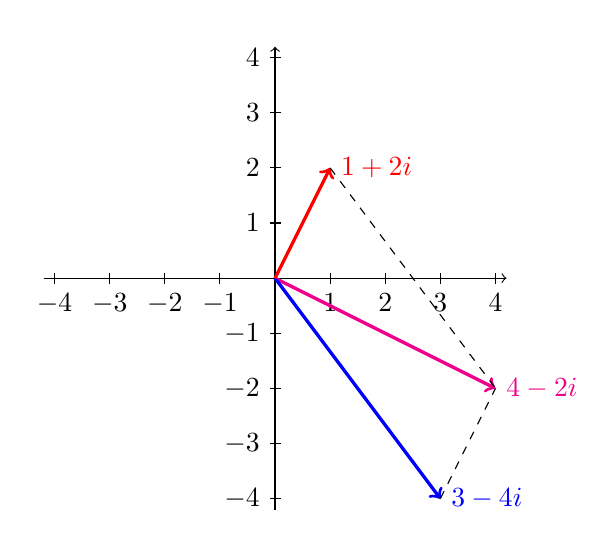
\begin{tikzpicture}[scale=.7]
\draw[arrows=->] (-4.2,0) -- (4.2,0) node[right] {$\R$};
\draw[arrows=->] (0,-4.2) -- (0,4.2) node[above] {$\R$};
 \foreach \pos in {-4,-3,-2,-1,1,2,3,4}
    \draw[shift={(\pos,0)}] (0,.1) -- (0,-.1) node[below] {$\pos$};
 \foreach \pos in {-4,-3,-2,-1,1,2,3,4}
    \draw[shift={(0,\pos)}] (.1,0) -- (-.1,0) node[left] {$\pos$};
\draw[magenta,very thick,arrows=->] (0,0)--(4,-2) node[right] {$4-2i$};
\draw[blue,very thick,arrows=->] (0,0)--(3,-4) node[right] {$3-4i$};
\draw[red,very thick,arrows=->] (0,0)--(1,2) node[right] {$1+2i$};
\draw[dashed] (3,-4)--(4,-2);
\draw[dashed] (1,2)--(4,-2);
\end{tikzpicture}
\end{center}
\end{ejemplo}

\subsection{Módulo de un número complejo}

Dado que estamos representando los números complejos como puntos en el plano; más aún, los estamos representando como flechas que van desde el origen hasta un determinado punto del plano, entonces puede ser interesante conocer el tamaño de esa flecha, en otras palabras, nos interesará conocer la distancia del origen del sistema cartesiano al punto que representa a $z$; tal magnitud la llamaremos \emph{módulo de $z$}. 

\medskip

\begin{defn}
    Dado un n\'umero complejo $z$, $z = a+ib $ con $a,b \in \R$, 
	se define el {\em m\'odulo de $z$} como el n\'umero real
	$$|z| = \sqrt{a^2+b^2}=\sqrt{(\textrm{Re}(z))^2+(\textrm{Im}(z))^2}.$$
\end{defn}
Recordemos que, si $z= a+ib$ es un complejo no nulo, entonces,
\begin{equation}\label{moduloconj}
	z^{-1} = \frac{a}{a^2+b^2}-i\frac{b}{a^2+b^2} = \frac{\left(a-ib\right)}{a^2+b^2}= \frac{\overline{z}}{|z|^2}.
\end{equation}
Esto es una interesante justificación para la introducción del concepto de conjugado.

\medskip

\begin{prop}
Dados dos complejos $z$, $w\in\C$ cualesquiera, se cumplen las siguientes propiedades.
\begin{enumerate}
\item $|z|\ge0$
\item $|z|=0$ si y solo si $z=0$
\item $|z|^2=z\overline{z}$
\item $|zw|=|z|\ |w|$
\item $|z^{-1}|=(|z|)^{-1}$
\item $|z+w|\le|z|+|w|$ {\bf (Desigualdad triangular)}
\item $|z|=|\overline{z}|$
\end{enumerate}
\end{prop}
{\bf Demostración.}
\begin{enumerate}
	\item 	
	En efecto, si $z=a+ib$, con $a,b\in\R$, entonces $|z|=\sqrt{a^2+b^2}$, y como $a,b\in\R$, entonces $a^2,b^2\ge 0$, así $a^2+b^2\ge 0$ y la raíz cuadrada se puede calcular, y por definición es un número mayor o igual a 0.
	\item 
	En efecto, si $z=a+ib$, con $a,b\in\R$, entonces 	
$$|z|=\sqrt{a^2+b^2}=0\Leftrightarrow {a^2+b^2}=0\Leftrightarrow a^2=0\wedge b^2=0\Leftrightarrow a=0\wedge b=0\Leftrightarrow z=0.$$
	\item De la ecuación~(\ref{moduloconj}), se obtiene directamente.
	\item 
	En efecto, basta observar, gracias a \eqref{moduloconj}, que
    \[
		|z w|^2 = z w \overline{z w} = z w \overline{z}  \overline{w} = z \overline{z} w \overline{w}
			= |z|^2 |w|^2.
    \]		
	\item 	
	En efecto, si $w = z^{-1}$ se tiene entonces que
            $|z| |z^{-1}| = |z z^{-1}| = |1| = 1$, es decir,
            $\left|z^{-1}\right| = \dfrac{1}{|z|} = |z|^{-1}$.
	\item Esta desigualdad no es tan simple de demostrar.
	Haremos uso de las siguientes propiedades: 
	\begin{itemize}
        \item para todo n\'umero real $x$ se cumple que $x \le |x|$.
        \item para todo n\'umero complejo $z = x + i y$ se tiene que 
            \[
                |\mbox{Re}(z)| = |x| = \sqrt{x^2} \le \sqrt{x^2 + y^2} = |z|.
            \]
	\end{itemize}
    Entonces,        
	\begin{align*}
        |z+w|^2 &= (z+w)(\overline{z+w}) \\
        &= (z+w)(\overline{z} + \overline{w})\\
              &  = |z|^2 + z\overline{w} + w\overline{z} + |w|^2\\
            &= |z|^2 + z\overline{w} + \overline{z\overline{w}} + |w|^2\\
                &= |z|^2 + 2\mbox{Re}(z\overline{w}) + |w|^2\\
            &\le |z|^2 + 2|\mbox{Re}(z\overline{w})| + |w|^2 \\
            &\le |z|^2 + 2|z\overline{w}| + |w|^2\\
            &= |z|^2 + 2|z|\ |\overline{w}| + |w|^2\\
            &= |z|^2 + 2|z|\ |w| + |w|^2\\
            &= \left(|z| + |w|\right)^2.
	\end{align*}
    Dado que se trata de n\'umeros reales no negativos, podemos extraer raíz cuadrada y concluir que:
    $$|z+w| \le |z| + |w|.$$
	\item 	
	En efecto, si $z=a+ib$, con $a,b\in\R$, entonces $\overline{z}=a-ib$, por lo tanto $|\overline{z}|=\sqrt{a^2+(-b)^2}=\sqrt{a^2+b^2}=|z|$.
\end{enumerate}

La última propiedad se visualiza en la siguiente figura, junto con la propiedad $|-z|=|z|$ la cual se obtiene de las anteriores tomando $w=-1$.

\begin{center}
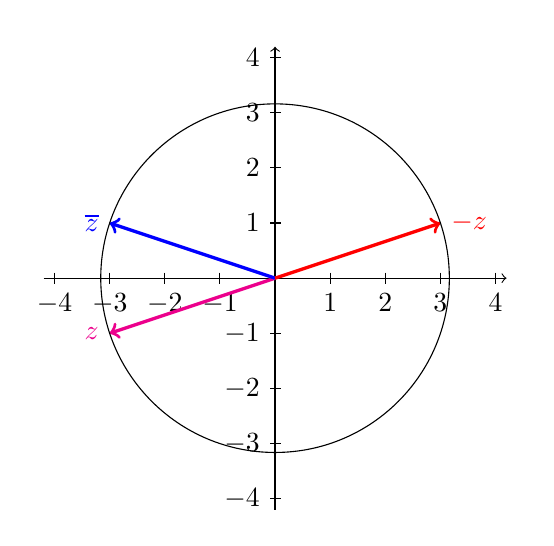
\begin{tikzpicture}[scale=.7]
\draw[arrows=->] (-4.2,0) -- (4.2,0) node[right] {$\R$};
\draw[arrows=->] (0,-4.2) -- (0,4.2) node[above] {$\R$};
 \foreach \pos in {-4,-3,-2,-1,1,2,3,4}
    \draw[shift={(\pos,0)}] (0,.1) -- (0,-.1) node[below] {$\pos$};
 \foreach \pos in {-4,-3,-2,-1,1,2,3,4}
    \draw[shift={(0,\pos)}] (.1,0) -- (-.1,0) node[left] {$\pos$};
\draw[magenta,very thick,arrows=->] (0,0)--(-3,-1) node[left] {$z$};
\draw[blue,very thick,arrows=->] (0,0)--(-3,1) node[left] {$\overline{z}$};
\draw[red,very thick,arrows=->] (0,0)--(3,1) node[right] {$-z$};
\draw (0,0) circle (3.1623);
\end{tikzpicture}
\end{center}

La propiedades previas nos permiten hacer cálculos complicados sin necesidad de conocer la parte real o imaginaria del número, tal como el siguiente ejercicio muestra.

\begin{ejercicio}
Demuestre que:
$$\forall \in\C\setminus\{0\},\ \left|\dfrac{|z|}{z}-\overline{z}\right|=|1-|z|\, |.$$
En efecto, 
\begin{eqnarray*}
\left|\dfrac{|z|}{z}-\overline{z}\right|&=&\left|\dfrac{|z|-z\overline{z}}{z}\right|\\
&=&\left|\dfrac{|z|-|z|^2}{z}\right|\\
&=&\left|\dfrac{|z|(1-|z|)}{z}\right|\\
&=&|z|\left|\dfrac{1-|z|}{z}\right|\\
&=&|z|\dfrac{|1-|z||}{|z|}\\
&=&|1-|z| |
\end{eqnarray*}
\end{ejercicio}


%%%%%%%%%%%%%%%%%%%%%%%%%%%%%%%%%%%%%%%%%%%%%%%%%%%%%%%%%%%%%
%
%  forma polar
%
%%%%%%%%%%%%%%%%%%%%%%%%%%%%%%%%%%%%%%%%%%%%%%%%%%%%%%%%%%%%%

\section{Forma polar}

Valiéndonos de lo que aprendimos en trigonometría, podemos representar un número complejo $z$ en el plano cartesiano (o Plano de Argand) a través de su módulo, $|z|$, y del ángulo $\theta$ entre la semirecta positiva
del eje real y el vector asociado a $z$.

\begin{center}
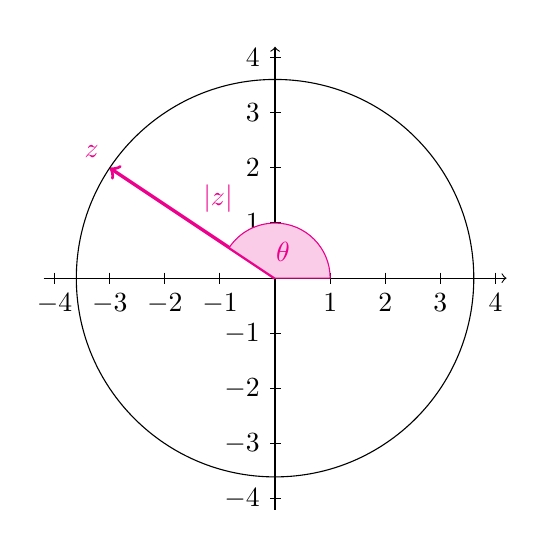
\begin{tikzpicture}[scale=.7]
\draw[arrows=->] (-4.2,0) -- (4.2,0) node[right] {$\R$};
\draw[arrows=->] (0,-4.2) -- (0,4.2) node[above] {$\R$};
 \foreach \pos in {-4,-3,-2,-1,1,2,3,4}
    \draw[shift={(\pos,0)}] (0,.1) -- (0,-.1) node[below] {$\pos$};
 \foreach \pos in {-4,-3,-2,-1,1,2,3,4}
    \draw[shift={(0,\pos)}] (.1,0) -- (-.1,0) node[left] {$\pos$};
\draw[magenta,very thick,arrows=->] (0,0)-- (-1.5,1) node[above right] {$|z|$} -- (-3,2) node[above left] {$z$};
\draw (0,0) circle (3.6056);
\filldraw[fill=magenta!20,draw=magenta]
    (0,0) -- (1,0) arc (0:146.31:1) -- cycle;
\node[magenta] at (73.15:.5) {$\theta$};
\end{tikzpicture}
\end{center}

Entonces si $z=x+iy$ tenemos que:

\[
    x = |z| \cos(\theta),\qquad y = |z| \sen(\theta)
\]
y as\'i podemos escribir:
\begin{equation}\label{polar1}
    z = x + i y = |z| \cos(\theta) + i |z| \sen(\theta) = |z| \big(\cos(\theta) + i \sen(\theta)\big),
\end{equation}
siendo \'esta \'ultima la {\em representaci\'on
polar de $z$}, cuando $z \ne 0$.

Observe que, debido a la periodicidad de las funciones
seno y coseno, el n\'umero 
\[
    z = |z| \big(\cos(\theta) + i \sen(\theta)\big)
\]
tambi\'en podr\'ia ser escrito como 
\[
    z = |z| \big(\cos(\theta +2 \pi\big) + i \sen(\theta + 2 \pi)\big)
\]
o, de forma m\'as general, como 
\[
    z = |z| \big(\cos(\theta +2 k \pi) + 
    i \sen(\theta+2 k \pi)\big),\qquad k \in \Z.
\]

Para evitar que haya infinitas formas de representar a un n\'umero complejo
en forma polar, el valor de $\theta$ en la representaci\'on polar
de $z$ se restringe al intervalo $=\left]-\pi,\pi\right]$. 
Esto motiva la siguiente definici\'on.

\medskip 

\begin{defn}{}{}
Dado $z\neq 0$, se definen
\begin{itemize}
\item \textit{argumento de $z$}, que se denota $\text{arg}(z)$, como 
    el conjunto de todos los ángulos que definen $z$, es decir,
    $$\arg(z)=\big\{\theta\in\mathbb{R}:
         z=|z| \big(\cos(\theta)+i \sen(\theta)\big)\big\},$$
\item \textit{el argumento principal de $z$}, 
    denotado $\text{Arg}(z)$, como el \'unico     
    argumento de $z$ que pertenece al intervalo $]-\pi,\pi]$.
\end{itemize}
Si $z=0$, entonces decimos que $\arg(z)$ y $\text{Arg}(z)$ {\bf son indeterminados}.
\end{defn}


\medskip


\begin{prop}
    Para todo $z\in\mathbb{C}\setminus\{0\}$, se cumple:
    $$\arg(z)=\big\{\text{Arg}(z)+2 k \pi: k\in\mathbb{Z}\big\}.$$
\end{prop}

En la expresi\'on de un n\'umero complejo $z \ne 0$ en forma polar $z = |z| \big(\cos(\theta) + i \sen(\theta)\big)$
la suma $\cos(\theta) + i \sen(\theta)$ se abrevia como $\textrm{cis}(\theta)$ y, con esto, $z$ se re -- escribe como
\[
    z = |z| \mbox{cis}(\theta).
\]

Ya hemos practicado en las Evaluaciones 1 y 2 cómo determinar el ángulo entre un segmento y uno de los semiejes cartesianos, esto lo practicaremos muchísimo en este capítulo, veamos un ejemplo.

\begin{ejemplo}{}{}
Dado $z = 1 + i$ un n\'umero en forma binomial. 
            Para escribirlo en forma polar debemos determinar $|z|$ y
            Arg$(z)$,
            $$|z| = |1+i| = \sqrt{1+1} = \sqrt{2}.$$					
            Dado que el par ordenado $(1,1)$ asociado a $z$ 
            est\'a en el primer cuadrante,
            \[
                \mbox{Arg}(z) = \mbox{Arctan}(\frac{1}{1}) = \frac{\pi}{4}\in]-\pi,\pi].
            \]
            La representaci\'on polar de $z$ es entonces
            \[
                z = \sqrt{2}\left(\cos\left(\frac{\pi}{4}\right) + 
                    i \sen\left(\frac{\pi}{4}\right)\right)
                    = \sqrt{2}\ \mbox{cis}\left(\frac{\pi}{4}\right). 
            \]
\end{ejemplo}

\begin{ejemplo}{}{}
Dado $z = -3 i$ un imaginario puro ubicado en la parte  negativa del eje imaginario,
            \[
                \mbox{Arg}(z) = -\frac{\pi}{2},\quad |z| = 3
                \qquad \mbox{ y } \qquad
                z = 3 \mbox{cis}\left(-\frac{\pi}{2}\right).
            \]
\end{ejemplo}


\subsection{Igualdad en forma polar}

Dados $z_1 = |z_1| \mbox{cis}(\theta_1)$ y $z_2 = |z_2| \mbox{cis}(\theta_2)$,
se cumple que 
\begin{equation}\label{igualdadpolar}
    z_1 = z_2 \quad \gdw \quad |z_1| = |z_2| \quad \wedge \quad \exists k\in\Z,\ \theta_1 = \theta_2+2 k \pi.
\end{equation}

Por ejemplo,
\[
    2 \mbox{cis}\left(\frac{\pi}{6}\right)=
     2 \mbox{cis}\left(\frac{-23\pi}{6}\right)
\]

\subsection{Conjugado en forma polar}
Dado $z = |z| \mbox{cis}(\theta)$, entonces $\overline{z} = |z| \mbox{cis}(-\theta)$.

En efecto, como $z= |z| \cos(\theta) + i |z| \sen(\theta)$, entonces 
\begin{eqnarray*}
|z| \cos(-\theta) + i |z| \sen(-\theta)&=& |z| \cos(\theta) - i |z| \sen(\theta)\\
&=&\overline{z}.
\end{eqnarray*}

\subsection{Opuesto aditivo en forma polar}
Dado $z = |z| \mbox{cis}(\theta)$, entonces $-z = |z| \mbox{cis}(\theta+\pi)$.

En efecto, como $z= |z| \cos(\theta) + i |z| \sen(\theta)$, entonces 
\begin{eqnarray*}
|z| \cos(\theta+\pi) + i |z| \sen(\theta+\pi)&=& -|z| \cos(\theta) - i |z| \sen(\theta)\\
&=&-z.
\end{eqnarray*}

Observe que el valor $\theta+\pi$ puede no ser el argumento principal de $- z$.


\subsection{Inverso multiplicativo en forma polar}
Dado $z = |z| \mbox{cis}(\theta)\not=0$, entonces $z^{-1} = \frac{1}{|z|} \mbox{cis}(-\theta)$.

En efecto, ya vimos que si $z \ne 0$, su inverso multiplicativo es el n\'umero complejo
$$z^{-1} = \frac{1}{|z|^2}\overline{z}.$$
Como $z = |z| \mbox{cis}(\theta)$, entonces
\begin{eqnarray*}
    z^{-1} &=& \frac{1}{|z|^2} \overline{z}\\
        &=& \frac{1}{|z|^2}  |z| \mbox{cis}(- \theta)\\
        & =& \frac{1}{|z|} \mbox{cis}(- \theta).
\end{eqnarray*}




Consideremos $z_1 = |z_1| \mbox{cis}(\theta_1)$ y $z_2 = |z_2| \mbox{cis}(\theta_2)$ en $\C$.

\subsection{Multiplicación en forma polar}

La {\bf suma} no tiene una expresión simple en la forma polar, de hecho no es fácil calcular el argumento de la suma de dos complejos a partir del argumento de los sumandos

Sin embargo, es la {\bf mutiplicación} la que hace realmente interesante a la forma polar.
Desarrollemos:
\begin{eqnarray*}
    z_1 z_2 &=& (|z_1| \mbox{cis}(\theta_1))(|z_2| \mbox{cis}(\theta_2))\\
    &=& |z_1| (\cos(\theta_1)+i \sen(\theta_1))|z_2| (\cos(\theta_2)+i \sen(\theta_2))\\
    &=& |z_1| |z_2| \big[\cos(\theta_1) \cos(\theta_2)-\sen(\theta_1) \sen(\theta_2)
    + i \big(\sen(\theta_1) \cos(\theta_2) + \cos(\theta_1) \sen(\theta_2)\big)\big],\\
\end{eqnarray*}
Pero esta expresión con productos de senos y cosenos está relacionada con el coseno $\cos(\theta_1+\theta_2)$ y $\sen(\theta_1+\theta_2)$, tal como establece el siguiente teorema.

\medskip

\begin{thm}
Dados dos ángulos cuales quiera $\theta_1$, $\theta_2\in\R$, se cumple:
$$\cos(\theta_1+\theta_2)=\cos(\theta_1) \cos(\theta_2)-\sen(\theta_1) \sen(\theta_2)\textrm{ y }\sen(\theta_1+\theta_2)=\sen(\theta_1) \cos(\theta_2) + \cos(\theta_1) \sen(\theta_2)$$
\end{thm}
{\bf Demostración} La siguiente figura es una prueba gráfica para el caso en que tanto $\theta_1$, $\theta_2$ como $\theta_1+\theta_2$ están $[0,\pi/2]$.

\begin{center}
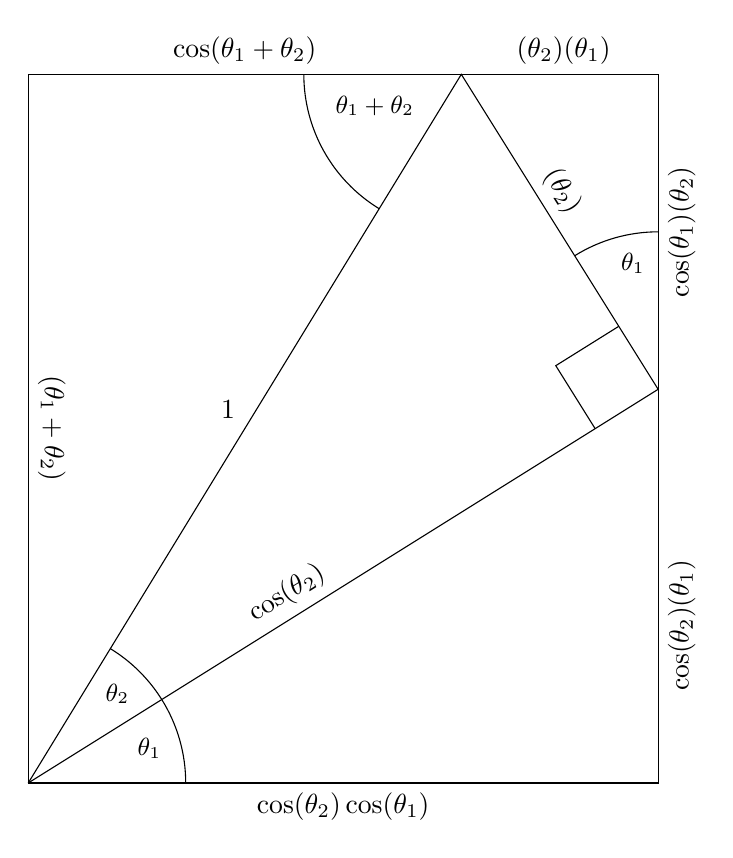
\begin{tikzpicture}[scale=2]
\draw (0,0) -- (4,0) node[midway,below] {$\cos(\theta_2)\cos(\theta_1)$}--(4,4.5) -- (0,4.5)--
	cycle node[midway,sloped,above]  {$\sen(\theta_1+\theta_2)$};
\draw (0,0) -- (4,2.5) node[midway,above left,sloped] {$\cos(\theta_2)$};
\node[below,rotate=90] at (4,1) {$\cos(\theta_2)\sen(\theta_1)$};
\draw (4,2.5)--(2.75,4.5) node[midway,above left,sloped] {$\sen(\theta_2)$}--(0,0) node[midway,above left] {1};
\node[below,rotate=90] at (4,3.5) {$\cos(\theta_1)\sen(\theta_2)$};
\node[above] at (3.4,4.5) {$\sen(\theta_2)\sen(\theta_1)$};
\draw (3.75,2.9)--++(-.4,-.25)--++(.25,-.4);
\draw (4,3.5) arc (90:122.005:1);
\node at (3.84,3.3) {\small$\theta_1$};
\draw (1,0) arc (0:32.005:1);
\node at (16:.8) {\small$\theta_1$};
\draw (32.005:1) arc (32.005:58.570:1);
\node at (45:.8) {\small$\theta_2$};
\node[above] at (1.375,4.5) {$\cos(\theta_1+\theta_2)$};
\draw (1.75,4.5) arc (180:238.57:1);
\node at (2.2,4.3) {\small$\theta_1+\theta_2$};
\end{tikzpicture}
\end{center}

Los demás casos se pueden obtener con bastante trabajo usando las simetrías e identidades vistas al comienzo del curso.
\hfill $\Box$

Esto da lugar a la siguiente hermosa y sintética fórmula.
\begin{eqnarray*}
   z_1 z_2  &=& |z_1| |z_2| \big(\cos(\theta_1+\theta_2)+i \sen(\theta_1+\theta_2)\big)\\
    &=& |z_1| |z_2| \mbox{cis}(\theta_1+\theta_2).
\end{eqnarray*}
También la división funciona muy bien.
\begin{align*}
    \frac{z_1}{z_2} &=  \frac{|z_1|}{|z_2|} \mbox{cis}(\theta_1-\theta_2).				
\end{align*}
Esto da una representaci\'on gr\'afica para el producto $z_1z_2$, usando trigonometría y triángulos semejantes.
\begin{ejemplo}
    Calculemos $z_1 z_2$ con
    \[
        z_1 = - \sqrt{3}+i,\qquad z_2 =\frac{1+ i}{2}.
    \]
    Dado que 
    \[
        z_1 = 2 \mbox{cis}\left(\frac{5 \pi}{6}\right),\qquad
        z_2 = \frac{\sqrt{2}}{2}\mbox{cis}\left(\frac\pi 4\right),
    \]
    su producto puede calcularse como 
    $$z_1 z_2 = \sqrt{2}\ \mbox{cis}\left(\frac{5 \pi}{6}+\frac\pi 4\right)=  \sqrt{2}\ \mbox{cis}\left(\frac{13 \pi}{12}\right)= 
         \sqrt{2}\ \mbox{cis}\left(-\frac{11 \pi}{12}\right).$$
        
\begin{center}
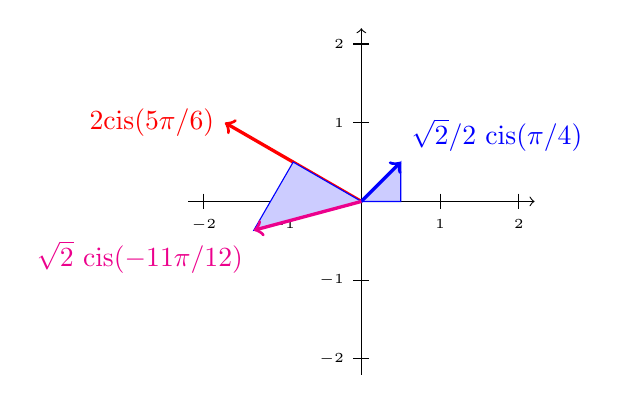
\begin{tikzpicture}
\draw[arrows=->] (-2.2,0) -- (2.2,0);
\draw[arrows=->] (0,-2.2) -- (0,2.2);
 \foreach \pos in {-2,-1,1,2}
    \draw[shift={(\pos,0)}] (0,.1) -- (0,-.1) node[below] {\tiny $\pos$};
 \foreach \pos in {-2,-1,1,2}
    \draw[shift={(0,\pos)}] (.1,0) -- (-.1,0) node[left] {\tiny $\pos$};

\draw[red,very thick,arrows=->] (0,0)-- (150:2)  node[left] {$2 \textrm{cis}(5\pi/6)$};
\filldraw[fill=blue!20!white,draw=blue]
    (0,0) -- (0.5,0) -- (45:0.7071) -- cycle;

\draw[blue,very thick,arrows=->] (0,0)-- (45:0.7071)  node[above right] {$\sqrt{2}/2\ \textrm{cis}(\pi/4)$};
\filldraw[fill=blue!20!white,draw=blue]
    (0,0) -- (150: 1) -- (195:1.4142) -- cycle;

\draw[magenta,very thick,arrows=->] (0,0)-- (-165:1.4142)  node[below left] {$\sqrt{2}\ \textrm{cis}(-11\pi/12)$};
\end{tikzpicture}
\end{center}


\end{ejemplo}

\subsection{Teorema de De Moivre: cálculo de potencias en forma polar} 

Dado que la multiplicación se simplifica tanto con la forma polar, lo mismo ocurre con las potencias enteras.		
Dados $z \in \C$ y $n \in \N$, la potencia con exponente natural $n$ de $z$ resulta tener la siguiente fórmula.

$$    z^n = |z|^n \mbox{cis}(n \theta).$$
    
La cual recibe el nombre de {\em F\'ormula de De Moivre}.
    
 La demostración se hace formalmente por inducción, pero proviene directamente de la fórmula de la multiplicación, en la cual el módulo de la multiplicación es la multiplicación de los módulos y el argumento de la multiplicación es la suma de los argumentos.

\begin{ejemplo}{}{}
    Calculemos  $(1+i)^4$.
    
    \begin{itemize}
        \item Podemos utilizar la f\'ormula del binomio,
        \[
            (1+i)^4 = 1 + 4 i + 6 i^2 + 4 i^3 + i^4 = 
                1 + 4 i - 6 - 4 i + 1 = - 4.
        \]
        
        \item Podemos escribir a $1+i$ en forma polar y utilizar la f\'ormula anterior
        \[
            1 + i = \sqrt{2} \mbox{cis}\left(\frac{\pi}{4}\right) 
            \quad \Longrightarrow \quad (1+i)^4 = 
            \big( \sqrt{2} \big)^4 \mbox{cis}\left(4 \frac{\pi}{4}\right) 
            = 4 \mbox{cis}(\pi)
            =4 \cos(\pi) + 4 i \sin(\pi) = - 4
        \]
        Comprobamos que llegamos al mismo resultado
    \end{itemize}
        
    La siguiente figura muestra sucesivamente: $(1+i)^{-1}$, $(1+i)^{0}$, $(1+i)$, $(1+i)^{2}$, $(1+i)^{3}$, $(1+i)^{4}$.
        
\begin{center}
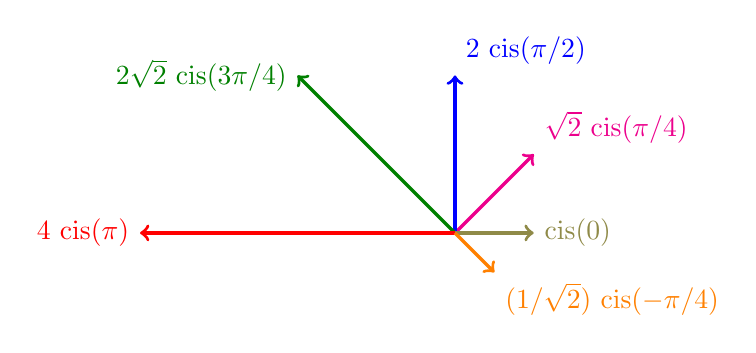
\begin{tikzpicture}

\draw[magenta,very thick,arrows=->] (0,0)-- (45:1.4142)  node[above right] {$\sqrt{2}\ \textrm{cis}(\pi/4)$};
\draw[blue,very thick,arrows=->] (0,0)-- (90:2)  node[above right] {$2\ \textrm{cis}(\pi/2)$};
\draw[green!50!black,very thick,arrows=->] (0,0)-- (135:2.8284)  node[left] {$2\sqrt{2}\ \textrm{cis}(3\pi/4)$};
\draw[red,very thick,arrows=->] (0,0)-- (180:4)  node[left] {$4\ \textrm{cis}(\pi)$};
\draw[yellow!50!black,very thick,arrows=->] (0,0)-- (0:1)  node[right] {$\textrm{cis}(0)$};
\draw[orange,very thick,arrows=->] (0,0)-- (-45:0.7071)  node[below right] {$(1/\sqrt{2})\ \textrm{cis}(-\pi/4)$};
\end{tikzpicture}
\end{center}


    
\end{ejemplo}

\medskip 


Análogamente, $z^{-n}$ puede calcularse mediante
\[
    \left(z^{-1}\right)^n = 
    \left(\left( |z| \mbox{cis}(\theta) \right)^{-1}\right)^n
    = \left(\frac{1}{|z|} \mbox{cis}(- \theta)\right)^n
    = \frac{1}{|z|^n} \mbox{cis}(- n \theta)=|z|^{-n} \mbox{cis}(- n \theta).
\]


\begin{ejercicio}{}{}
    Calcule y escriba el resultado en forma polar de $(1+\sqrt{3} i)^{200}$.
    
\begin{eqnarray*}
(1+\sqrt{3} i)^{200} &=& \left(2 \mbox{cis}\left(\frac \pi 3\right)\right)^{200}\\
            &=& 2^{200} \mbox{cis}\left(\frac{200\pi}{3}\right)\\
            &=& 2^{200}\mbox{cis}\left(\frac{(3\cdot 66 + 1) \pi}{3}\right)\\
                &=& 2^{200}\mbox{cis}\left(66 \pi + \frac{\pi}{3}\right)\\
                &=& 2^{200}\mbox{cis}\left(33\cdot 2 \pi + \frac{\pi}{3}\right)\\
                &=& 2^{200}\mbox{cis}\left(\frac{\pi}{3}\right)
\end{eqnarray*}
\end{ejercicio}

\section{Ra\'ices de un número complejo}


En los reales solo considerábamos la raíz cuadrada positiva de un número positivo, descartando su opuesto aditivo que sin embargo daba el mismo resultado al elevarse al cuadrado. 
En el conjunto de los números complejos nos abriremos a considerar varias raíces, partiendo de la siguiente definición.

\begin{defn}{}{}
Dado $z \in \C$, y $n \in \N$, decimos que $w\in\C$ es una  {\em ra\'{\i}z $n$-\'esima de $z$}
si cumple que $w^n = z$.
\end{defn}


Con esta definición tanto 2 como -2 son raíces cuadradas de 4, ya no hablamos de \emph{la} raíz de 4 sino de \emph{las} raíces.


También tenemos que tanto $i$ como $-i$ son raíces cuadradas de $-1$.
Por lo tanto vemos también que tanto $1$ como $-1$, $i$ y $-i$ sin todas raíces cuartas de $1$, ya que 

$$ 1^4=(-1)^4=i^4=(-i)^4=1.$$

Por otra parte, observamos que solo 0 es raíz de 0, este número tiene solo una raíz.

?`C\'omo determinar una ra\'iz $n$-\'esima $w$ de un $z$ dado?
Hay muchas maneras, pero dado que fue sencillo calcular las potencias de un número en forma polar, será también sencillo calcular sus raíces en forma polar, veamos.
Supongamos que 
$z = |z| \mbox{cis}(\theta_z)$ y queremos determinar 
$w$ en forma polar $|w| \mbox{cis}(\theta_w)$ de manera tal que $w^n = z$.
 
Como $w^n = |w|^n \mbox{cis}(n \theta_w)=|z| \mbox{cis}(\theta_z)$,
se cumple si y s\'olo si,
\begin{align*}
    |w|^n=|z| \textrm{ y existe } k\in \Z \textrm{ tal que } n \theta_w=\theta_z +2k\pi,
\end{align*}
o, equivalentemente,
\begin{align*}
    |w|=\sqrt[n]{|z|} \textrm{ y existe } k\in \Z \textrm{ tal que } \theta_w=\frac{\theta_z}{n} +\frac{ 2 k  \pi}{n}
\end{align*}
de manera que en principio no hay una si no infinitas raíces... pero ¿será realmente así? ¿qué pasa cuando tomamos $k=n$?
$$\theta_w=\frac{\theta_z}{n} +\frac{ 2 n  \pi}{n}=\frac{\theta_z}{n}+2 \pi$$
el cual es equivalente al argumento $\dfrac{\theta_z}{n}$, el cual se obtiene tomando $k=0$.

En general tendremos que tomar $k+n$ es equivalente a tomar $k$, así $z$ solo tiene $n$ raíces:
\begin{align*}
    w_k=\sqrt[n]{|z|} cis \left(\frac{\theta_z}{n} +\frac{ 2 k  \pi}{n}\right), \textrm{ con } k\in\{0,1,\dots,n-1\}
\end{align*}

Lo anterior permite inferir el siguiente resultado:

\begin{lem}{}{}
    Para todo $z \in \C$, $z\neq 0$, se cumple que 
    $z$ tiene $n$ ra\'{\i}ces $n$-\'esimas distintas entre s\'{\i}. 
    Si $z = |z| \mbox{cis}(\theta)$, entonces estas son:
    \begin{equation}\label{raicesz}
        \left\{
            |z|^{1/n} \mbox{cis}\left(\frac{\theta}{n} + 
            \frac{2 j \pi}{n}\right)\;:\;
            j \in \{0,1,2,\ldots, n-1\}
        \right\}
    \end{equation}
\end{lem}


\begin{prueba}
    Seg\'un se vio antes, las ra\'ices $n$-\'esimas de 
    $z = |z| \mbox{cis}(\theta)$ son los
    n\'umeros complejos de la forma
    \[
       |z|^{\frac 1 n} 
            \mbox{cis}\left(\frac{\theta}{n} + 2 \pi \frac{k}{n}
            \right)\;:\; k \in \Z
    \]
    Cualquier n\'umero natural $k$ deja resto entre 0 y $n-1$ al dividirlo por $n$, por tanto,
    cualquer n\'umero entero $k$ puede escribirse
    como 
    \[
        k = m n + j,\qquad \mbox{ con } m \in \Z \quad \wedge \quad j \in \{0,1,2,\cdots,n-1\}.
    \]
    Entonces, las ra\'ices $n$ -- \'esimas de $z$ están dadas por:
    \[
        \left\{|z|^{\frac 1 n} \mbox{cis}\left(\frac{\theta}{n} + 
            2 \pi \frac{m n+j}{n}\right)\;:\;m \in \Z \quad \wedge \quad j \in \{0,1,2,\cdots,n-1\}\right\}.
    \]
    Reemplazando $m$ por $0$ se obtienen los valores en \eqref{raicesz}. 
    Ahora, para cada $j \in \{0,1,2,\ldots,n-1\}$ sea 
    $w_j = |z|^{1/n} \mbox{cis}\left(\frac{\theta}{n} + \frac{2 j \pi}{n}\right)$,
    con lo cual se obtiene la siguiente descomposici\'on,
    \[
            \underbrace{\left\{w_0,  w_1,  \cdots,  w_{n-1}\right\}}_{=: {\mathcal R}_1}
            \;\bigcup\; 
            \underbrace{\left\{|z|^{\frac 1 n} \mbox{cis}\left(\frac{\theta}{n} + 
            2 \pi \frac{m n+j}{n}\right)\;:\; m \in \Z-\{0\} \quad \wedge \quad
            j \in \{0,1,2,\cdots,n-1\}\right\}}_{=: {\mathcal R}_2}.
    \]    
    Si $w \in {\mathcal R}_2$, existen $m \in \Z-\{0\}$ y $j \in \{0,1,\cdots,n-1\}$
    de modo que 
    \[
       w = |z|^{\frac 1 n} \mbox{cis}\left(\frac{\theta}{n} + 
            2 \pi \frac{m n+j}{n}\right)
            =
            |z|^{\frac 1 n} \mbox{cis}\left(\frac{\theta}{n} + 2 \pi m + 2 \pi \frac{j}{n}\right).
    \]
    Debido a que las funciones seno y coseno son peri\'odicas de per\'iodo
    $2 \pi$ se tiene que 
    \[
        w = |z|^{\frac 1 n} \mbox{cis}\left(\frac{\theta}{n} + 2 \pi m + 2 \pi \frac{j}{n}\right)
        = |z|^{\frac 1 n} \mbox{cis}\left(\frac{\theta}{n} + 2 \pi \frac{j}{n}\right)
        = w_j.
    \]
    Es decir, cada elemento $w \in {\mathcal R}_2$ es igual a alguno de los $n$ elementos
    en ${\mathcal R}_1$, y as\'i, las ra\'ices $n$ -- \'esimas de $z$ es,
    por tanto, el conjunto ${\mathcal R}_1$.   
\end{prueba}



\begin{ejemplo}{}{}
    Calculemos las ra\'{\i}ces cuadradas de $1+i\sqrt{3} =  2 \mbox{cis}\left(\frac \pi 3\right)$.
        
    Los n\'umeros complejos de la forma
    \[
        2^{1/2} \mbox{cis}\left(\frac \pi 6 + k \pi\right)
    \]
    con $k \in \{0,1\}$ son ra\'ices cuadradas de $1+i\sqrt{3}$. 
     
    Demos valores a $k$ y veamos qu\'e n\'umeros complejos   son ra\'ices cuadradas de $1 +i \sqrt{3}$.    
    \begin{itemize}
        \item con $k = 0$: $\sqrt{2} \mbox{cis}\left(\frac \pi 6\right)$. 
            Llam\'emosle $w_0$.
            
        \item con $k = 1$: 
            $\sqrt{2} \mbox{cis}\left(\frac \pi 6 + \pi\right) =
            \sqrt{2} \mbox{cis}\left(\frac{7 \pi}{6}\right) = 
            \sqrt{2} \mbox{cis}\left(-\frac{5 \pi}{6}\right)$.
            Llam\'emosle $w_1$.
       \item con $k=2$: $\sqrt{2} \mbox{cis}\left(\frac \pi 6 + 2 \pi\right)$,
            que es igual al valor que obtuvimos con $k=0$,
            es decir, es igual a $w_0$.
       \item con $k = 3$:  $\sqrt{2} \mbox{cis}\left(\frac \pi 6 + 3 \pi\right)
            = \sqrt{2} \mbox{cis}\left(\frac \pi 6 + \pi\right) 
            = \sqrt{2} \mbox{cis}\left(\frac \pi 6 + \pi - 2 \pi\right)$,
            y es igual al valor que obtuvimos con $k=1$, que denominamos
            $w_1$.
    \end{itemize}
    Por lo tanto $1+i\sqrt{3}$ tiene solo dos raíces cuadradas: $w_0$ y $w_1$.
    
    
\begin{center}
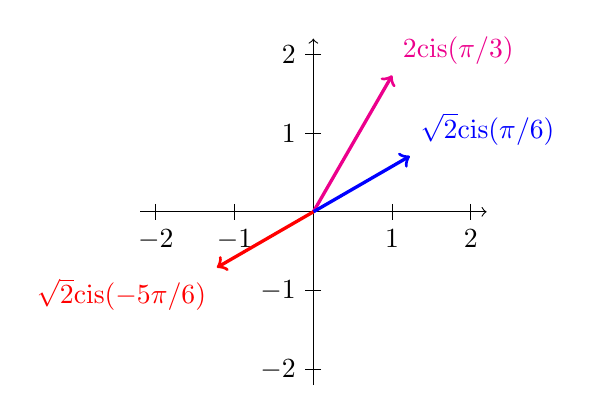
\begin{tikzpicture}
\draw[arrows=->] (-2.2,0) -- (2.2,0);
\draw[arrows=->] (0,-2.2) -- (0,2.2);
 \foreach \pos in {-2,-1,1,2}
    \draw[shift={(\pos,0)}] (0,.1) -- (0,-.1) node[below] {$\pos$};
 \foreach \pos in {-2,-1,1,2}
    \draw[shift={(0,\pos)}] (.1,0) -- (-.1,0) node[left] {$\pos$};
\draw[magenta,very thick,arrows=->] (0,0)-- (60:2)  node[above right] {$2\textrm{cis}(\pi/3)$};
\draw[blue,very thick,arrows=->] (0,0)-- (30:1.4142)  node[above right] {$\sqrt{2}\textrm{cis}(\pi/6)$};
\draw[red,very thick,arrows=->] (0,0)-- (-150:1.4142)  node[below left] {$\sqrt{2}\textrm{cis}(-5\pi/6)$};
\end{tikzpicture}
\end{center}
\end{ejemplo}     
               
\begin{ejemplo}{}{} 
    Determinemos las ra\'{\i}ces cuartas de 
    $i = \mbox{cis}\left(\frac \pi 2 \right)$.
    
    De lo anterior, tenemos que estas son:
    $$w = \mbox{cis}\left(\frac \pi 8 + \frac{2k \pi}{ 4} \right)= \mbox{cis}\left(\frac \pi 8 + k\frac \pi 2 \right),$$    
    con $k$ tomando valores $0, 1, 2, 3$.
    \begin{align*}
        w_0 &= \mbox{cis}\left(\frac \pi 8\right)\; &\mbox{ con } 
        k &= 0,\\
        w_1 &= \mbox{cis}\left(\frac{5 \pi}{8}\right)\; &\mbox{ con } 
        k &= 1,\\
        w_2 &= \mbox{cis}\left(\frac{9 \pi}{8}\right) =
            \mbox{cis}\left(-\frac{7 \pi}{8}\right),\; &\mbox{con } 
            k &= 2,\\
        w_3 &= \mbox{cis}\left(\frac{13 \pi}{8}\right) =
            \mbox{cis}\left(-\frac{3 \pi}{8}\right),\; &\mbox{ con  } 
            k &= 3.
    \end{align*}
    
\begin{center}
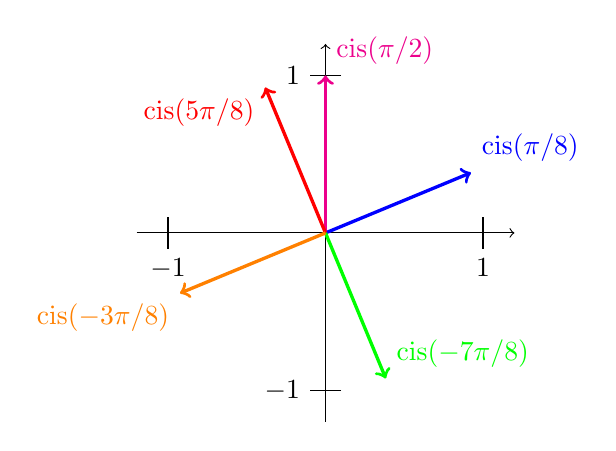
\begin{tikzpicture}[scale=2]
\draw[arrows=->] (-1.2,0) -- (1.2,0);
\draw[arrows=->] (0,-1.2) -- (0,1.2);
 \foreach \pos in {-1,1}
    \draw[shift={(\pos,0)}] (0,.1) -- (0,-.1) node[below] {$\pos$};
 \foreach \pos in {-1,1}
    \draw[shift={(0,\pos)}] (.1,0) -- (-.1,0) node[left] {$\pos$};
\draw[magenta,very thick,arrows=->] (0,0)-- (90:1)  node[above right] {$\textrm{cis}(\pi/2)$};
\draw[blue,very thick,arrows=->] (0,0)-- (22.5:1)  node[above right] {$\textrm{cis}(\pi/8)$};
\draw[red,very thick,arrows=->] (0,0)-- (112.5:1)  node[below left] {$\textrm{cis}(5\pi/8)$};
\draw[green,very thick,arrows=->] (0,0)-- (-67.5:1)  node[above right] {$\textrm{cis}(-7\pi/8)$};
\draw[orange,very thick,arrows=->] (0,0)-- (-157.5:1)  node[below left] {$\textrm{cis}(-3\pi/8)$};
\end{tikzpicture}
\end{center}

\end{ejemplo}

Los reales también adquirirán muchas raíces nuevas según esta nueva definición, en general, todo numero, real o complejo, tendrá exactamente $n$ raíces $n$-ésimas distintas.
En particular las raíces $n$-ésimas de $z=1$ son:
$$ u_k=\mbox{cis}\left(\frac{2k\pi}{n}\right),\textrm{ con }k\in\{0,1,\dots,n-1\}.$$


\begin{center}
\begin{tikzpicture}
  \draw[arrows=->,color=blue!50!red] (-6,0) -- ++ (120:2);
  \draw[arrows=->,color=blue!50!red] (-6,0) -- ++(0:2);
  \draw[arrows=->,color=blue!50!red] (-6,0) -- ++ (-120:2);
  \node at (-6,3) {Las 3 raíces 3-ésimas de 1};


  \draw[arrows=->,color=blue!50!red] (0,0) -- ++ (90:2);
  \draw[arrows=->,color=blue!50!red] (0,0) -- ++(0:2);
  \draw[arrows=->,color=blue!50!red] (0,0) -- ++ (-90:2);
  \draw[arrows=->,color=blue!50!red] (0,0) -- ++ (180:2);
  \node at (0,3) {Las 4 raíces 4-ésimas de 1};

  
  \draw[arrows=->,color=blue!50!red] (6,0) -- ++ (72:2);
  \draw[arrows=->,color=blue!50!red] (6,0) -- ++(0:2);
  \draw[arrows=->,color=blue!50!red] (6,0) -- ++ (144:2);
  \draw[arrows=->,color=blue!50!red] (6,0) -- ++ (-144:2);
  \draw[arrows=->,color=blue!50!red] (6,0) -- ++ (-72:2);
  \node at (6,3) {Las 5 raíces 5-ésimas de 1};
\end{tikzpicture}
\end{center}

Pasa un fenómeno muy interesante cuando sumamos las $n$-ésimas raíces de la unidad:

\begin{center}
\begin{tikzpicture}
  \draw[arrows=->,color=blue!50!red] (-6,0) -- ++(0:2)-- ++ (120:2)-- ++ (-120:2);

  \draw[arrows=->,color=blue!50!red] (0,0) -- ++(0:2)-- ++ (90:2) -- ++ (180:2)-- ++ (-90:2);
 

  
  \draw[arrows=->,color=blue!50!red] (6,0) -- ++(0:2)-- ++ (72:2)-- ++ (144:2)-- ++(-144:2)-- ++ (-72:2);
\end{tikzpicture}
\end{center}

¡¡Las raíces $n$-ésimas de la unidad conforman un polígono regular de $n$ lados!! y dado que se trata de un polígono cerrado, su suma es cero siempre. 

Pero lo más interesante es las raíces de 1 es que nos permiten obtener las raíces de todos los demás números complejos.
\begin{lem}{}{}
    Sean $n\in\N$ y $z \in \C$ tal que $z=|z|\mbox{cis}(\theta_z) \ne 0$, y sean $u_0,\dots , u_{n-1}$ las raíces $n$-ésimas de 1.
    Entonces, las ra\'{\i}ces $n$ -- \'esimas de $z$ son:
    \[
        \sqrt[n]{|z|} \mbox{cis}\left(\frac{\theta_z}{n}\right)u_0,\sqrt[n]{|z|} \mbox{cis}\left(\frac{\theta_z}{n}\right) u_1,  \cdots, \sqrt[n]{|z|} \mbox{cis}\left(\frac{\theta_z}{n}\right)u_{n-1}.
    \]
\end{lem}



\begin{prueba}
Sabemos que las raíces $n$-ésimas de $z$ son:
$$\sqrt[n]{|z|} \mbox{cis}\left(\frac{\theta_z}{n}+\frac{2 k \pi}{n}\right),\mbox{ con } k\in\{0,1,\dots,n-1\}$$
Sea $k\in\{0,1,\dots,n-1\}$ fijo, observemos lo siguiente:
$$\sqrt[n]{|z|} \mbox{cis}\left(\frac{\theta_z}{n}+\frac{2 k \pi}{n}\right)=\sqrt[n]{|z|} \mbox{cis}\left(\frac{\theta_z}{n}\right)\mbox{cis}\left(\frac{2 k \pi}{n}\right)=\sqrt[n]{|z|} \mbox{cis}\left(\frac{\theta_z}{n}\right)u_k$$
Con lo cual queda demostrado lo afirmado.
\end{prueba}

\begin{center}
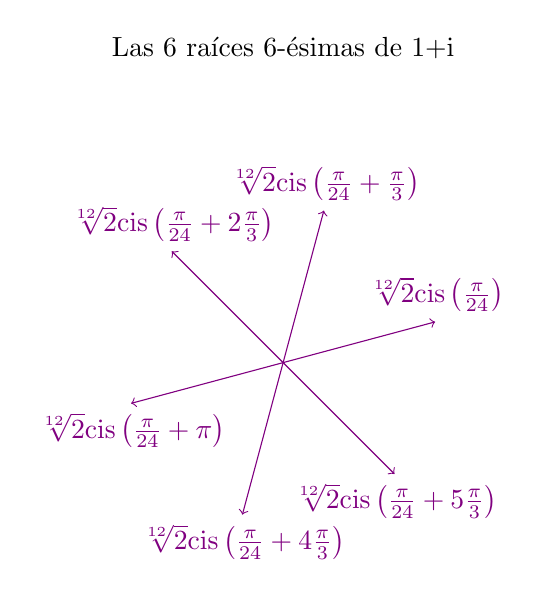
\begin{tikzpicture}
  \draw[arrows=->,color=blue!50!red] (0,0) -- ++ (15:2) node[above] {$\sqrt[12]{2}\mbox{cis}\left(\frac{\pi}{24}\right)$};
  \draw[arrows=->,color=blue!50!red] (0,0) -- ++ (75:2) node[above] {$\sqrt[12]{2}\mbox{cis}\left(\frac{\pi}{24}+\frac{\pi}{3}\right)$};
  \draw[arrows=->,color=blue!50!red] (0,0) -- ++(135:2) node[above] {$\sqrt[12]{2}\mbox{cis}\left(\frac{\pi}{24}+2\frac{\pi}{3}\right)$};
  \draw[arrows=->,color=blue!50!red] (0,0) -- ++ (195:2) node[below] {$\sqrt[12]{2}\mbox{cis}\left(\frac{\pi}{24}+\pi\right)$};
  \draw[arrows=->,color=blue!50!red] (0,0) -- ++ (255:2) node[below] {$\sqrt[12]{2}\mbox{cis}\left(\frac{\pi}{24}+4\frac{\pi}{3}\right)$};
  \draw[arrows=->,color=blue!50!red] (0,0) -- ++ (315:2) node[below] {$\sqrt[12]{2}\mbox{cis}\left(\frac{\pi}{24}+5\frac{\pi}{3}\right)$};
  \node at (0,4) {Las 6 raíces 6-ésimas de 1+i};
 \end{tikzpicture}
\end{center}

\medskip

\begin{cor}{}{}
    Para todo n\'umero complejo $z$ se cumple que la suma de sus 
    ra\'{\i}ces $n$ -- \'esimas es cero.
\end{cor}

\subsection{Ejercicios}

Terminamos este apunte con dos ejercicios.

\begin{ejercicio}{}{}
    \begin{enumerate}
        \item Resuelva en $\C$ y en $\R$ la ecuaci\'on $x^2 + 2x + 4 = 0$.
        \item Resuelva en $\C$ la ecuaci\'on 
        $\displaystyle z^2 + \frac 1 z = 0$.
    \end{enumerate}
    \vspace{0.3cm}
    \textbf{Soluci\'on:}
    \begin{enumerate}
        \item 
            Procedamos a completar cuadrados.
            \begin{align*}
                0 = x^2 + 2 x + 4\quad & \gdw \quad 0 = (x^2 + 2 x + 1) + 4 - 1
                \quad \gdw \quad (x+1)^2 = - 3,
            \end{align*}
            Si $x \in \R$, entonces $(x+1)^2 \ge 0$ y 
            la ecuaci\'on anterior
            no tiene soluci\'on.\\
            
            Si $x \in \C$, la ecuaci\'on $(x+1)^2 = - 3$ 
            es equivalente a que 
            $x+1$ sea una de las ra\'ices cuadradas de $- 3$, es decir, dado que $- 3=3\mbox{cis}(\pi)$
            \begin{align*}
                x+1 \in &\left\{ \sqrt{3}\mbox{cis}\left(\frac{\pi}{2}\right),\sqrt{3}\mbox{cis}\left(\frac{\pi}{2}+\frac{2\pi}{2}\right)\right\}\\
                =&\left\{ \sqrt{3}\mbox{cis}\left(\frac{\pi}{2}\right),\sqrt{3}\mbox{cis}\left(\frac{\pi}{2}+\pi\right)\right\}\\
                =&\left\{ \sqrt{3}i,-\sqrt{3}i\right\}
            \end{align*}
            El conjunto de todos
            los n\'umeros complejos que elevarlos al cuadrado dan
            $- 3$ es aqu\'el formado por los complejos 
            $\sqrt{3} i$ y $-\sqrt{3} i$.\\
            
            Por tanto, las soluciones de la ecuaci\'on dada son	
            $- 1 + \sqrt{3} i$ y $- 1 - \sqrt{3} i$, lo cual coincide con la fórmula que ya teníamos del liceo (verificar).
            
        \item Si $z \in \C \setminus \{0\}$,
            \begin{align*}
                z^2 + \frac 1 z = 0 \quad \gdw \quad \frac{z^3 + 1}{z} = 0 \quad \gdw \quad z^3 + 1 = 0 \quad \gdw \quad z 
                \in \sqrt[3]{- 1}
            \end{align*}
            Entonces, las soluciones de la ecuaci\'on dada son las ra\'{\i}ces c\'ubicas de
            $- 1 = \mbox{cis}(\pi)$.
    \end{enumerate}
\end{ejercicio}


